%% ============================================================================
%%  Can Ambient WiFi Replace LiDAR for Automotive SLAM?
%%  Localization Yes, Mapping No --- and Why
%%
%%  Target venue: IEEE Internet of Things Journal (IoT-J). IEEEtran journal class.
%%  Build:  pdflatex main && bibtex main && pdflatex main && pdflatex main
%%          (IEEEtran.cls/.bst vendored; no siunitx dependency) or use Overleaf.
%%
%%  EVERY quantitative claim is reproduced from a committed artifact in data/.
%%  See README.md for the section -> data-file provenance table.
%% ============================================================================
\documentclass[journal]{IEEEtran}

\usepackage{amsmath,amssymb}
\usepackage{graphicx}
\usepackage{booktabs}
\usepackage{url}
\usepackage[hidelinks]{hyperref}
\usepackage{tikz}
\usetikzlibrary{arrows.meta,positioning,fit,backgrounds,calc}
\graphicspath{{../../docs/assets/}}

% Lightweight unit macros (self-contained; equivalent to siunitx \SI/\SIrange/\num
% output but with no external dependency, so the paper builds anywhere).
\newcommand{\SI}[2]{#1\,#2}
\newcommand{\SIrange}[3]{#1--#2\,#3}
\newcommand{\num}[1]{#1}
\newcommand{\si}[1]{#1}
\providecommand{\degree}{\ensuremath{^\circ}}

% No-op fallbacks for IEEEtran bibliography spacing macros.
\providecommand{\BIBdecl}{}
\providecommand{\BIBentrySTDinterwordspacing}{}
\providecommand{\BIBentryALTinterwordspacing}{}
\providecommand{\BIBentryALTinterwordstretchfactor}[1]{}
\providecommand{\BIBforeignlanguage}[2]{#2}

\begin{document}

\title{Can Ambient WiFi Replace LiDAR for Automotive SLAM?\\
Localization Yes, Mapping No --- and Why}

\author{Mulham~Fetna%
\thanks{M.~Fetna is an independent researcher (e-mail: contact@mulhamfetna.com;
ORCID 0009-0006-4432-798X).}%
\thanks{Code, data, and every figure-generating script are released openly;
all reported numbers are reproduced from the committed artifacts.}}

\markboth{IEEE Internet of Things Journal}%
{Fetna: Can Ambient WiFi Replace LiDAR for Automotive SLAM?}

\maketitle

\begin{abstract}
LiDAR dominates the sensor cost of an autonomous vehicle, which motivates a blunt
question: can ambient WiFi sensing simply take its place? We answer it with the first
head-to-head, on-vehicle, outdoor comparison of WiFi and LiDAR SLAM evaluated on the
\emph{same} ray-traced scenes, against the \emph{same} ground truth, with the
\emph{same} six metrics. The study is simulation-based (Sionna RT), anchored by a
real-LiDAR control: our SLAM back-end run on KITTI odometry attains
\SI{1.16}{m} aligned ATE over a \SI{394}{m} drive ($\approx0.3\%$ drift), which is
consistent with real LiDAR odometry. Three findings follow. First, on
\emph{localization} commodity-CSI WiFi is not merely competitive but superior: it
reaches \SI{0.027}{m} ATE, better than either of our LiDAR models, at
\textbf{84--600$\times$} lower sensor cost. Second, on \emph{mapping} it fails outright
(occupancy IoU $\approx 0$ versus up to $1.00$ for LiDAR), and no price buys coverage it
cannot produce. Third, we locate the mapping ceiling precisely: it is \emph{not} path
discrimination, as previously supposed, but a front-end limit --- roughly
\textbf{89\%} of MUSIC detections correspond to \emph{no real propagation path}, and a
\SI{6.45}{m} median range \emph{bias} (far beyond the \SI{0.94}{m} resolution limit)
corrupts the rest. Consequently a learned discriminator cannot repair the map, and we
show that a heuristic, a random forest, and a neural network all fail identically. The
practical consequence is a hybrid: adding WiFi to an existing LiDAR costs
$\approx0.5\%$ more and improves localization by \textbf{36--79\%} --- provided the two
sensors are of comparable accuracy, since a badly mismatched pair degrades the stronger
one.
\end{abstract}

\begin{IEEEkeywords}
Internet of Things, SLAM, Wi-Fi, channel state information, LiDAR, sensor fusion,
autonomous vehicles, cost analysis, ray tracing.
\end{IEEEkeywords}

\section{Introduction}

\IEEEPARstart{L}{iDAR} is the reference exteroceptive sensor for vehicle SLAM, and it is
also the expensive one: a mid-range spinning unit of the class routinely used in
research costs thousands of dollars, while the WiFi silicon already present in a
vehicle costs tens. If ambient WiFi --- signals that are radiated anyway, by
infrastructure that already exists --- could stand in for LiDAR, the sensing bill for
autonomy would change by orders of magnitude. That is the question this paper asks, and
it asks it without hedging: \emph{can WiFi replace LiDAR, or not?}

The honest answer turns out to be neither ``yes'' nor ``no'' but a boundary, and the
boundary is the contribution. WiFi replaces LiDAR for one half of SLAM and fails at the
other, and the failure is not where the literature --- including our own earlier work
\cite{fetna2026wifiradar} --- assumed it was.

\subsection{Contributions}

\begin{enumerate}
\item \textbf{The first on-vehicle, outdoor, head-to-head WiFi-vs-LiDAR SLAM
comparison.} Both modalities are evaluated on identical ray-traced scenes against
identical footprint ground truth with an identical metric suite, and the LiDAR
back-end is externally validated on real KITTI data \cite{geiger2012kitti}
($\approx0.3\%$ drift). Prior WiFi-SLAM is indoor \cite{arun2022p2slam}, or uses WiFi
to \emph{assist} a primary ranging sensor \cite{arun2022viwid,ismail2022wifilidarslam};
none tests replacement on a vehicle (Section~\ref{sec:related}).

\item \textbf{A sensor-cost analysis} --- to our knowledge the first for WiFi-vs-LiDAR
SLAM --- including \emph{cost-normalized} accuracy and coverage. WiFi's sensing package
is \textbf{84--600$\times$} cheaper than the LiDAR class we simulate, and delivers two
to three orders of magnitude better accuracy per dollar (Section~\ref{sec:cost}).

\item \textbf{A symmetric fusion study with a cost verdict.} Fusing the two helps
\emph{conditionally}, and we identify the condition (sensor parity): fusion beats both
solo sensors in three of four configurations but \emph{degrades} the stronger sensor by
$8\times$ when the pair is badly mismatched (Section~\ref{sec:fusion}).

\item \textbf{The mapping ceiling, located.} An isolation experiment shows the WiFi
mapping floor is dominated by \emph{phantom} detections ($\approx89\%$) and estimator
\emph{range bias}, not by path discrimination. This refines the interpretation of
\cite{fetna2026wifiradar} and tells a learned method where it must act
(Section~\ref{sec:ceiling}).
\end{enumerate}

\subsection{Relationship to our prior work}
This paper extends \cite{fetna2026wifiradar}, which established ambient WiFi as a
feasible \emph{radar}-replacement sensing front-end and reported an oracle-sensing map
at \SI{0.25}{m} accuracy alongside a realistic-sensing map bounded near \SI{5}{m}. Its
empirical results are reused here, not re-derived. Section~\ref{sec:ceiling} refines one
of its \emph{interpretations}: that work attributed the realistic-mapping floor to path
discrimination and argued the discrimination was learnable. The isolation experiment
below shows discrimination is in fact the \emph{smallest} of three mechanisms, and that
a learned discriminator therefore cannot lift the map.

\section{Related Work}\label{sec:related}

\textbf{WiFi as a standalone SLAM sensor.} P2SLAM \cite{arun2022p2slam} is the closest
prior art: it extracts two-way bearings from commodity CSI and integrates them with
odometry in a GraphSLAM back-end, achieving \SI{26.9}{cm} median tracking. It is,
however, evaluated \emph{indoors only} ($25\times30$\,m and $50\times40$\,m, with fixed
anchors) and is benchmarked against \emph{visual} SLAM, not LiDAR. Radio-fingerprint
SLAM \cite{liu2023radiofingerprintslam} does run outdoors on a mobile platform and uses
radio as the primary modality, but it relies on RSS fingerprinting from smartphones
rather than CSI, runs on a slow research UGV rather than a road vehicle, and attains its
best accuracy only when fused with LiDAR.

\textbf{WiFi as an assistant to a primary sensor.} A larger body of work uses WiFi to
\emph{augment} a ranging sensor rather than replace it. ViWiD \cite{arun2022viwid}
offloads loop closure from a visual back-end to WiFi; \cite{ismail2022wifilidarslam}
supplies WiFi fingerprint loop closures to a LiDAR SLAM that still performs the mapping;
\cite{li2025ekfwifilidarimu} fuses WiFi RSSI, LiDAR and IMU in an EKF. In every case
LiDAR or a camera remains the mapping sensor. None of these works reports a WiFi-vs-LiDAR
SLAM accuracy comparison, and none treats WiFi as a candidate replacement.

\textbf{Learned RF sensing.} Deep models can recover geometry from RF: RF-Pose
\cite{zhao2018rfpose} estimates human pose through walls from WiFi-band reflections,
\cite{geng2022denseposewifi} regresses dense body pose from commodity CSI, and
\cite{maatta2024csipointcloud} reconstructs 3-D point clouds from CSI with a transformer.
Notably these methods learn \emph{end-to-end from raw CSI}; none classifies estimated
propagation paths. Section~\ref{sec:ceiling} explains why that distinction is decisive.

\textbf{The open cell.} On-vehicle, outdoor, commodity-CSI WiFi sensing evaluated
head-to-head against LiDAR for SLAM --- with a cost analysis --- is, to our knowledge,
unoccupied. This paper occupies it.

\section{System Model}\label{sec:method}

Both modalities are driven through one pipeline and scored on one plane, so that any
difference between them is attributable to the sensor and not to the estimator, the
scene, or the metric (Fig.~\ref{fig:system}).

\textbf{Scenes and ground truth.} Two ray-traced outdoor scenes are used throughout: a
\emph{controlled wall} (a large metal reflector, giving clean single-bounce geometry)
and a reflective \emph{street canyon} with buildings and cars. Ground truth is the
bird's-eye footprint of every non-floor scatterer, identical for both sensors.

\textbf{WiFi path.} Ambient access points illuminate the scene; the vehicle receives
commodity CSI, from which a joint 2-D (delay--azimuth) MUSIC front-end estimates each
path's bistatic delay and arrival azimuth. Each detection is triangulated on the bistatic
ellipse --- the reflector lies where the measured path length
$|\mathrm{AP}\!\rightarrow\!R| + |R\!\rightarrow\!\mathrm{veh}|$ and the arrival bearing
intersect --- and the resulting reflectors, together with the same detections used as
particle weights, drive a Rao-Blackwellized particle-filter SLAM.

\textbf{LiDAR path.} The LiDAR is reduced to the same plane: a horizontal ring produces a
2-D scan, which a scan-to-map ICP registers against an accumulated voxel map. Because a
single LiDAR model would beg the question of \emph{which} LiDAR, we bracket the sensor
with two models (Section~\ref{sec:lidar}).

\textbf{The common comparison plane.} Trajectories are $xy$, maps are 2-D point sets, and
both sensors are scored with the same six metrics: ATE and RPE for the trajectory;
Chamfer distance, directional map-accuracy (estimate$\rightarrow$truth) and
map-completeness (truth$\rightarrow$estimate), and occupancy IoU for the map. Reducing
LiDAR to 2-D is a deliberate, stated choice: it is what makes the comparison
apples-to-apples, and it is discussed as a limitation in Section~\ref{sec:discussion}.

\begin{figure*}[t]
\centering
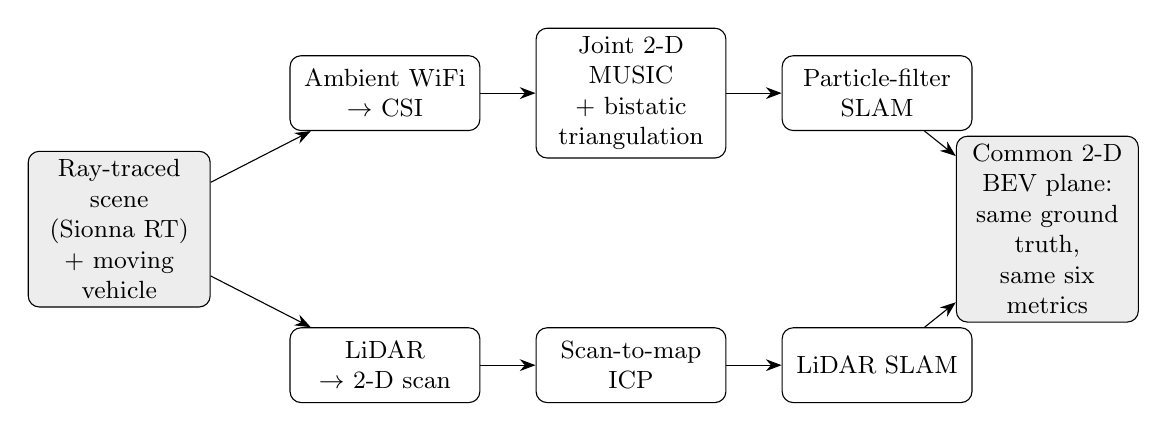
\begin{tikzpicture}[
  font=\small,
  block/.style={draw, rounded corners, minimum height=0.95cm, text width=2.2cm,
                align=center, inner sep=3pt},
  io/.style={draw, rounded corners, fill=black!7, minimum height=0.95cm,
             text width=2.1cm, align=center, inner sep=3pt},
  >={Stealth[length=2mm]}]
  \node[io] (scene) {Ray-traced scene\\ (Sionna RT)\\ + moving vehicle};
  \node[block, above right=0.25cm and 1.0cm of scene] (csi) {Ambient WiFi\\ $\rightarrow$ CSI};
  \node[block, below right=0.25cm and 1.0cm of scene] (scan) {LiDAR\\ $\rightarrow$ 2-D scan};
  \node[block, right=0.7cm of csi] (music) {Joint 2-D MUSIC\\ + bistatic\\ triangulation};
  \node[block, right=0.7cm of scan] (icp) {Scan-to-map\\ ICP};
  \node[block, right=0.7cm of music] (pf) {Particle-filter\\ SLAM};
  \node[block, right=0.7cm of icp] (lslam) {LiDAR SLAM};
  \node[io, right=1.0cm of $(pf)!0.5!(lslam)$] (out)
      {Common 2-D BEV plane:\\ same ground truth,\\ same six metrics};
  \draw[->] (scene) -- (csi);
  \draw[->] (scene) -- (scan);
  \draw[->] (csi) -- (music);
  \draw[->] (scan) -- (icp);
  \draw[->] (music) -- (pf);
  \draw[->] (icp) -- (lslam);
  \draw[->] (pf) -- (out);
  \draw[->] (lslam) -- (out);
\end{tikzpicture}
\caption{Both sensors are driven through the same scene and scored on the same 2-D
bird's-eye plane, against the same footprint ground truth, with the same six metrics.
Any difference is then attributable to the sensor, not to the estimator or the metric.}
\label{fig:system}
\end{figure*}

\end{document}
